\documentclass[1p]{elsarticle_modified}
%\bibliographystyle{elsarticle-num}

%\usepackage[colorlinks]{hyperref}
%\usepackage{abbrmath_seonhwa} %\Abb, \Ascr, \Acal ,\Abf, \Afrak
\usepackage{amsfonts}
\usepackage{amssymb}
\usepackage{amsmath}
\usepackage{amsthm}
\usepackage{scalefnt}
\usepackage{amsbsy}
\usepackage{kotex}
\usepackage{caption}
\usepackage{subfig}
\usepackage{color}
\usepackage{graphicx}
\usepackage{xcolor} %% white, black, red, green, blue, cyan, magenta, yellow
\usepackage{float}
\usepackage{setspace}
\usepackage{hyperref}

\usepackage{tikz}
\usetikzlibrary{arrows}

\usepackage{multirow}
\usepackage{array} % fixed length table
\usepackage{hhline}

%%%%%%%%%%%%%%%%%%%%%
\makeatletter
\renewcommand*\env@matrix[1][\arraystretch]{%
	\edef\arraystretch{#1}%
	\hskip -\arraycolsep
	\let\@ifnextchar\new@ifnextchar
	\array{*\c@MaxMatrixCols c}}
\makeatother %https://tex.stackexchange.com/questions/14071/how-can-i-increase-the-line-spacing-in-a-matrix
%%%%%%%%%%%%%%%

\usepackage[normalem]{ulem}

\newcommand{\msout}[1]{\ifmmode\text{\sout{\ensuremath{#1}}}\else\sout{#1}\fi}
%SOURCE: \msout is \stkout macro in https://tex.stackexchange.com/questions/20609/strikeout-in-math-mode

\newcommand{\cancel}[1]{
	\ifmmode
	{\color{red}\msout{#1}}
	\else
	{\color{red}\sout{#1}}
	\fi
}

\newcommand{\add}[1]{
	{\color{blue}\uwave{#1}}
}

\newcommand{\replace}[2]{
	\ifmmode
	{\color{red}\msout{#1}}{\color{blue}\uwave{#2}}
	\else
	{\color{red}\sout{#1}}{\color{blue}\uwave{#2}}
	\fi
}

\newcommand{\Sol}{\mathcal{S}} %segment
\newcommand{\D}{D} %diagram
\newcommand{\A}{\mathcal{A}} %arc


%%%%%%%%%%%%%%%%%%%%%%%%%%%%%5 test

\def\sl{\operatorname{\textup{SL}}(2,\Cbb)}
\def\psl{\operatorname{\textup{PSL}}(2,\Cbb)}
\def\quan{\mkern 1mu \triangleright \mkern 1mu}

\theoremstyle{definition}
\newtheorem{thm}{Theorem}[section]
\newtheorem{prop}[thm]{Proposition}
\newtheorem{lem}[thm]{Lemma}
\newtheorem{ques}[thm]{Question}
\newtheorem{cor}[thm]{Corollary}
\newtheorem{defn}[thm]{Definition}
\newtheorem{exam}[thm]{Example}
\newtheorem{rmk}[thm]{Remark}
\newtheorem{alg}[thm]{Algorithm}

\newcommand{\I}{\sqrt{-1}}
\begin{document}

%\begin{frontmatter}
%
%\title{Boundary parabolic representations of knots up to 8 crossings}
%
%%% Group authors per affiliation:
%\author{Yunhi Cho} 
%\address{Department of Mathematics, University of Seoul, Seoul, Korea}
%\ead{yhcho@uos.ac.kr}
%
%
%\author{Seonhwa Kim} %\fnref{s_kim}}
%\address{Center for Geometry and Physics, Institute for Basic Science, Pohang, 37673, Korea}
%\ead{ryeona17@ibs.re.kr}
%
%\author{Hyuk Kim}
%\address{Department of Mathematical Sciences, Seoul National University, Seoul 08826, Korea}
%\ead{hyukkim@snu.ac.kr}
%
%\author{Seokbeom Yoon}
%\address{Department of Mathematical Sciences, Seoul National University, Seoul, 08826,  Korea}
%\ead{sbyoon15@snu.ac.kr}
%
%\begin{abstract}
%We find all boundary parabolic representation of knots up to 8 crossings.
%
%\end{abstract}
%\begin{keyword}
%    \MSC[2010] 57M25 
%\end{keyword}
%
%\end{frontmatter}

%\linenumbers
%\tableofcontents
%
\newcommand\colored[1]{\textcolor{white}{\rule[-0.35ex]{0.8em}{1.4ex}}\kern-0.8em\color{red} #1}%
%\newcommand\colored[1]{\textcolor{white}{ #1}\kern-2.17ex	\textcolor{white}{ #1}\kern-1.81ex	\textcolor{white}{ #1}\kern-2.15ex\color{red}#1	}

{\Large $\underline{12n_{0281}~(K12n_{0281})}$}

\setlength{\tabcolsep}{10pt}
\renewcommand{\arraystretch}{1.6}
\vspace{1cm}\begin{tabular}{m{100pt}>{\centering\arraybackslash}m{274pt}}
\multirow{5}{120pt}{
	\centering
	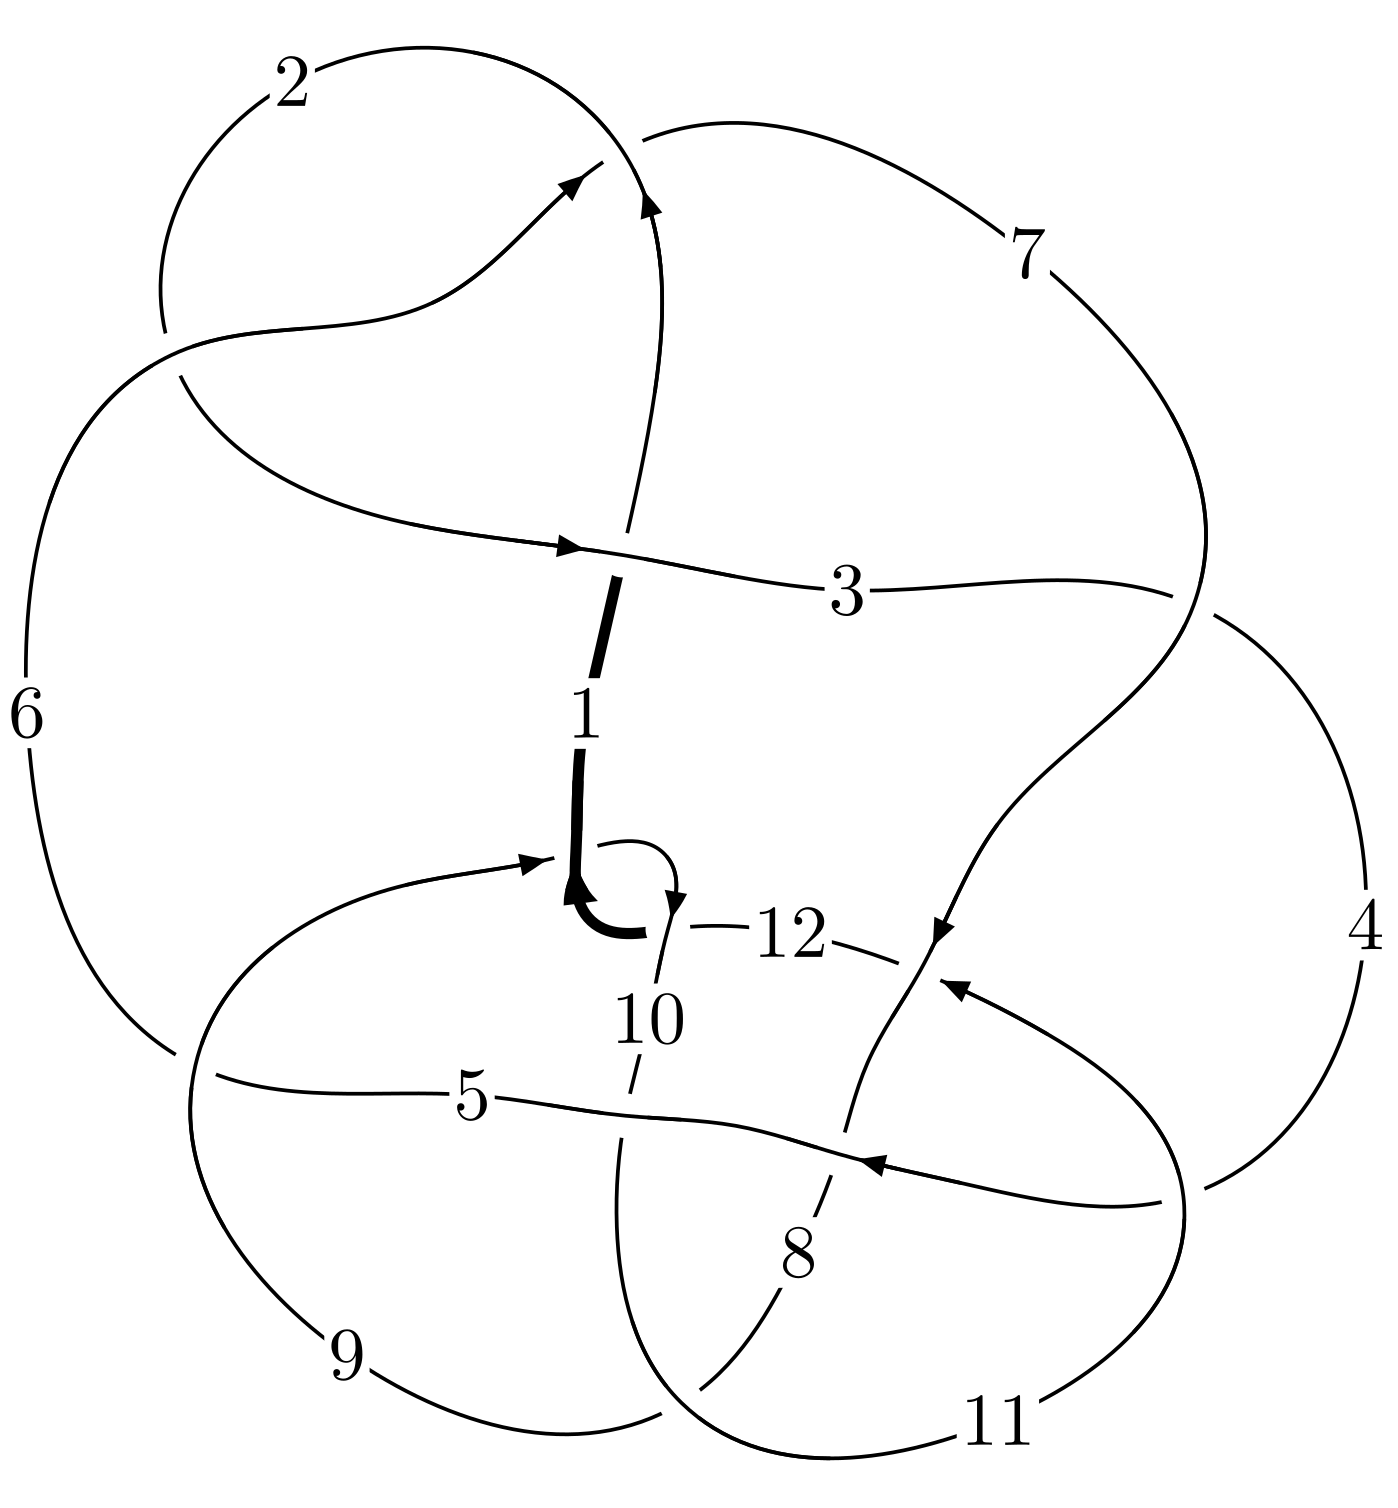
\includegraphics[width=112pt]{../../../GIT/diagram.site/Diagrams/png/2370_12n_0281.png}\\
\ \ \ A knot diagram\footnotemark}&
\allowdisplaybreaks
\textbf{Linearized knot diagam} \\
\cline{2-2}
 &
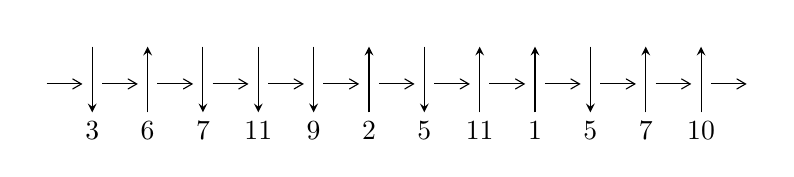
\begin{tikzpicture}[x=20pt, y=17pt]
	% nodes
	\node (C0) at (0, 0) {};
	\node (C1) at (1, 0) {};
	\node (C1U) at (1, +1) {};
	\node (C1D) at (1, -1) {3};

	\node (C2) at (2, 0) {};
	\node (C2U) at (2, +1) {};
	\node (C2D) at (2, -1) {6};

	\node (C3) at (3, 0) {};
	\node (C3U) at (3, +1) {};
	\node (C3D) at (3, -1) {7};

	\node (C4) at (4, 0) {};
	\node (C4U) at (4, +1) {};
	\node (C4D) at (4, -1) {11};

	\node (C5) at (5, 0) {};
	\node (C5U) at (5, +1) {};
	\node (C5D) at (5, -1) {9};

	\node (C6) at (6, 0) {};
	\node (C6U) at (6, +1) {};
	\node (C6D) at (6, -1) {2};

	\node (C7) at (7, 0) {};
	\node (C7U) at (7, +1) {};
	\node (C7D) at (7, -1) {5};

	\node (C8) at (8, 0) {};
	\node (C8U) at (8, +1) {};
	\node (C8D) at (8, -1) {11};

	\node (C9) at (9, 0) {};
	\node (C9U) at (9, +1) {};
	\node (C9D) at (9, -1) {1};

	\node (C10) at (10, 0) {};
	\node (C10U) at (10, +1) {};
	\node (C10D) at (10, -1) {5};

	\node (C11) at (11, 0) {};
	\node (C11U) at (11, +1) {};
	\node (C11D) at (11, -1) {7};

	\node (C12) at (12, 0) {};
	\node (C12U) at (12, +1) {};
	\node (C12D) at (12, -1) {10};
	\node (C13) at (13, 0) {};

	% arrows
	\draw[->,>={angle 60}]
	(C0) edge (C1) (C1) edge (C2) (C2) edge (C3) (C3) edge (C4) (C4) edge (C5) (C5) edge (C6) (C6) edge (C7) (C7) edge (C8) (C8) edge (C9) (C9) edge (C10) (C10) edge (C11) (C11) edge (C12) (C12) edge (C13) ;	\draw[->,>=stealth]
	(C1U) edge (C1D) (C2D) edge (C2U) (C3U) edge (C3D) (C4U) edge (C4D) (C5U) edge (C5D) (C6D) edge (C6U) (C7U) edge (C7D) (C8D) edge (C8U) (C9D) edge (C9U) (C10U) edge (C10D) (C11D) edge (C11U) (C12D) edge (C12U) ;
	\end{tikzpicture} \\
\hhline{~~} \\& 
\textbf{Solving Sequence} \\ \cline{2-2} 
 &
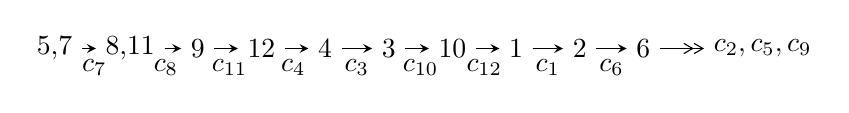
\begin{tikzpicture}[x=23pt, y=7pt]
	% node
	\node (A0) at (-1/8, 0) {5,7};
	\node (A1) at (17/16, 0) {8,11};
	\node (A2) at (17/8, 0) {9};
	\node (A3) at (25/8, 0) {12};
	\node (A4) at (33/8, 0) {4};
	\node (A5) at (41/8, 0) {3};
	\node (A6) at (49/8, 0) {10};
	\node (A7) at (57/8, 0) {1};
	\node (A8) at (65/8, 0) {2};
	\node (A9) at (73/8, 0) {6};
	\node (C1) at (1/2, -1) {$c_{7}$};
	\node (C2) at (13/8, -1) {$c_{8}$};
	\node (C3) at (21/8, -1) {$c_{11}$};
	\node (C4) at (29/8, -1) {$c_{4}$};
	\node (C5) at (37/8, -1) {$c_{3}$};
	\node (C6) at (45/8, -1) {$c_{10}$};
	\node (C7) at (53/8, -1) {$c_{12}$};
	\node (C8) at (61/8, -1) {$c_{1}$};
	\node (C9) at (69/8, -1) {$c_{6}$};
	\node (A10) at (11, 0) {$c_{2},c_{5},c_{9}$};

	% edge
	\draw[->,>=stealth]	
	(A0) edge (A1) (A1) edge (A2) (A2) edge (A3) (A3) edge (A4) (A4) edge (A5) (A5) edge (A6) (A6) edge (A7) (A7) edge (A8) (A8) edge (A9) ;
	\draw[->>,>={angle 60}]	
	(A9) edge (A10);
\end{tikzpicture} \\ 

\end{tabular} \\

\footnotetext{
The image of knot diagram is generated by the software ``\textbf{Draw programme}" developed by Andrew Bartholomew(\url{http://www.layer8.co.uk/maths/draw/index.htm\#Running-draw}), where we modified some parts for our purpose(\url{https://github.com/CATsTAILs/LinksPainter}).
}\phantom \\ \newline 
\centering \textbf{Ideals for irreducible components\footnotemark of $X_{\text{par}}$} 
 
\begin{align*}
I^u_{1}&=\langle 
1.82494\times10^{252} u^{57}+1.82764\times10^{251} u^{56}+\cdots+7.78104\times10^{252} b-1.44190\times10^{253},\\
\phantom{I^u_{1}}&\phantom{= \langle  }1.60321\times10^{253} u^{57}+2.56712\times10^{252} u^{56}+\cdots+7.78104\times10^{252} a-9.32328\times10^{253},\\
\phantom{I^u_{1}}&\phantom{= \langle  }u^{58}+51 u^{56}+\cdots-13 u+1\rangle \\
I^u_{2}&=\langle 
-6.06692\times10^{19} u^{19}+9.41482\times10^{19} u^{18}+\cdots+3.14683\times10^{19} b+6.57389\times10^{19},\\
\phantom{I^u_{2}}&\phantom{= \langle  }3.61452\times10^{19} u^{19}-9.01759\times10^{19} u^{18}+\cdots+3.14683\times10^{19} a-2.09263\times10^{20},\;u^{20}- u^{19}+\cdots+8 u+1\rangle \\
\\
\end{align*}
\raggedright * 2 irreducible components of $\dim_{\mathbb{C}}=0$, with total 78 representations.\\
\footnotetext{All coefficients of polynomials are rational numbers. But the coefficients are sometimes approximated in decimal forms when there is not enough margin.}
\newpage
\renewcommand{\arraystretch}{1}
\centering \section*{I. $I^u_{1}= \langle 1.82\times10^{252} u^{57}+1.83\times10^{251} u^{56}+\cdots+7.78\times10^{252} b-1.44\times10^{253},\;1.60\times10^{253} u^{57}+2.57\times10^{252} u^{56}+\cdots+7.78\times10^{252} a-9.32\times10^{253},\;u^{58}+51 u^{56}+\cdots-13 u+1 \rangle$}
\flushleft \textbf{(i) Arc colorings}\\
\begin{tabular}{m{7pt} m{180pt} m{7pt} m{180pt} }
\flushright $a_{5}=$&$\begin{pmatrix}0\\u\end{pmatrix}$ \\
\flushright $a_{7}=$&$\begin{pmatrix}1\\0\end{pmatrix}$ \\
\flushright $a_{8}=$&$\begin{pmatrix}1\\u^2\end{pmatrix}$ \\
\flushright $a_{11}=$&$\begin{pmatrix}-2.06041 u^{57}-0.329920 u^{56}+\cdots-90.1499 u+11.9821\\-0.234536 u^{57}-0.0234883 u^{56}+\cdots-14.4397 u+1.85309\end{pmatrix}$ \\
\flushright $a_{9}=$&$\begin{pmatrix}1.04387 u^{57}+0.167750 u^{56}+\cdots+52.9864 u-10.8517\\0.0421526 u^{57}+0.0173690 u^{56}+\cdots-0.700871 u-1.05817\end{pmatrix}$ \\
\flushright $a_{12}=$&$\begin{pmatrix}-2.29494 u^{57}-0.353409 u^{56}+\cdots-104.590 u+13.8351\\-0.234536 u^{57}-0.0234883 u^{56}+\cdots-14.4397 u+1.85309\end{pmatrix}$ \\
\flushright $a_{4}=$&$\begin{pmatrix}-1.79431 u^{57}-0.269090 u^{56}+\cdots-65.9513 u+8.42012\\-0.213324 u^{57}-0.0357409 u^{56}+\cdots-2.42241 u+1.31296\end{pmatrix}$ \\
\flushright $a_{3}=$&$\begin{pmatrix}-2.00763 u^{57}-0.304831 u^{56}+\cdots-68.3737 u+9.73308\\-0.213324 u^{57}-0.0357409 u^{56}+\cdots-2.42241 u+1.31296\end{pmatrix}$ \\
\flushright $a_{10}=$&$\begin{pmatrix}-2.06041 u^{57}-0.329920 u^{56}+\cdots-90.1499 u+11.9821\\-0.208881 u^{57}-0.0233171 u^{56}+\cdots-12.2111 u+1.52317\end{pmatrix}$ \\
\flushright $a_{1}=$&$\begin{pmatrix}-0.509191 u^{57}-0.192771 u^{56}+\cdots-58.2608 u+2.04977\\-0.241169 u^{57}-0.0405319 u^{56}+\cdots-13.7690 u+1.62656\end{pmatrix}$ \\
\flushright $a_{2}=$&$\begin{pmatrix}-0.507749 u^{57}+0.0273770 u^{56}+\cdots-44.2370 u+10.1377\\0.125301 u^{57}+0.0350847 u^{56}+\cdots+1.61989 u+0.441525\end{pmatrix}$ \\
\flushright $a_{6}=$&$\begin{pmatrix}1.13600 u^{57}+0.228021 u^{56}+\cdots+37.0000 u-3.53009\\0.207315 u^{57}+0.0430301 u^{56}+\cdots+3.66730 u-1.06964\end{pmatrix}$\\&\end{tabular}
\flushleft \textbf{(ii) Obstruction class $= -1$}\\~\\
\flushleft \textbf{(iii) Cusp Shapes $= -1.19694 u^{57}-0.252356 u^{56}+\cdots-49.4008 u+2.76120$}\\~\\
\newpage\renewcommand{\arraystretch}{1}
\flushleft \textbf{(iv) u-Polynomials at the component}\newline \\
\begin{tabular}{m{50pt}|m{274pt}}
Crossings & \hspace{64pt}u-Polynomials at each crossing \\
\hline $$\begin{aligned}c_{1}\end{aligned}$$&$\begin{aligned}
&u^{58}+28 u^{57}+\cdots+886 u+121
\end{aligned}$\\
\hline $$\begin{aligned}c_{2},c_{6}\end{aligned}$$&$\begin{aligned}
&u^{58}-2 u^{57}+\cdots-40 u+11
\end{aligned}$\\
\hline $$\begin{aligned}c_{3}\end{aligned}$$&$\begin{aligned}
&u^{58}+2 u^{57}+\cdots-2542 u+3839
\end{aligned}$\\
\hline $$\begin{aligned}c_{4},c_{10}\end{aligned}$$&$\begin{aligned}
&u^{58}- u^{57}+\cdots+10 u+1
\end{aligned}$\\
\hline $$\begin{aligned}c_{5}\end{aligned}$$&$\begin{aligned}
&u^{58}+3 u^{57}+\cdots+60 u+88
\end{aligned}$\\
\hline $$\begin{aligned}c_{7}\end{aligned}$$&$\begin{aligned}
&u^{58}+51 u^{56}+\cdots-13 u+1
\end{aligned}$\\
\hline $$\begin{aligned}c_{8}\end{aligned}$$&$\begin{aligned}
&u^{58}+3 u^{57}+\cdots+12935 u+481
\end{aligned}$\\
\hline $$\begin{aligned}c_{9},c_{12}\end{aligned}$$&$\begin{aligned}
&u^{58}+6 u^{57}+\cdots+289 u+41
\end{aligned}$\\
\hline $$\begin{aligned}c_{11}\end{aligned}$$&$\begin{aligned}
&u^{58}-3 u^{57}+\cdots-790066 u+205619
\end{aligned}$\\
\hline
\end{tabular}\\~\\
\newpage\renewcommand{\arraystretch}{1}
\flushleft \textbf{(v) Riley Polynomials at the component}\newline \\
\begin{tabular}{m{50pt}|m{274pt}}
Crossings & \hspace{64pt}Riley Polynomials at each crossing \\
\hline $$\begin{aligned}c_{1}\end{aligned}$$&$\begin{aligned}
&y^{58}+12 y^{57}+\cdots+130490 y+14641
\end{aligned}$\\
\hline $$\begin{aligned}c_{2},c_{6}\end{aligned}$$&$\begin{aligned}
&y^{58}+28 y^{57}+\cdots+886 y+121
\end{aligned}$\\
\hline $$\begin{aligned}c_{3}\end{aligned}$$&$\begin{aligned}
&y^{58}-4 y^{57}+\cdots-237147274 y+14737921
\end{aligned}$\\
\hline $$\begin{aligned}c_{4},c_{10}\end{aligned}$$&$\begin{aligned}
&y^{58}+75 y^{57}+\cdots-50 y+1
\end{aligned}$\\
\hline $$\begin{aligned}c_{5}\end{aligned}$$&$\begin{aligned}
&y^{58}-21 y^{57}+\cdots-103568 y+7744
\end{aligned}$\\
\hline $$\begin{aligned}c_{7}\end{aligned}$$&$\begin{aligned}
&y^{58}+102 y^{57}+\cdots-15 y+1
\end{aligned}$\\
\hline $$\begin{aligned}c_{8}\end{aligned}$$&$\begin{aligned}
&y^{58}-81 y^{57}+\cdots+2622113 y+231361
\end{aligned}$\\
\hline $$\begin{aligned}c_{9},c_{12}\end{aligned}$$&$\begin{aligned}
&y^{58}+22 y^{57}+\cdots+63341 y+1681
\end{aligned}$\\
\hline $$\begin{aligned}c_{11}\end{aligned}$$&$\begin{aligned}
&y^{58}-77 y^{57}+\cdots+288375606396 y+42279173161
\end{aligned}$\\
\hline
\end{tabular}\\~\\
\newpage\flushleft \textbf{(vi) Complex Volumes and Cusp Shapes}
$$\begin{array}{c|c|c}  
\text{Solutions to }I^u_{1}& \I (\text{vol} + \sqrt{-1}CS) & \text{Cusp shape}\\
 \hline 
\begin{aligned}
u &= -0.605403 + 0.770255 I \\
a &= \phantom{-}0.476324 - 1.234450 I \\
b &= -0.836696 - 0.528282 I\end{aligned}
 & -3.29534 - 3.17863 I & \phantom{-0.000000 } 0 \\ \hline\begin{aligned}
u &= -0.605403 - 0.770255 I \\
a &= \phantom{-}0.476324 + 1.234450 I \\
b &= -0.836696 + 0.528282 I\end{aligned}
 & -3.29534 + 3.17863 I & \phantom{-0.000000 } 0 \\ \hline\begin{aligned}
u &= \phantom{-}0.785984 + 0.673927 I \\
a &= \phantom{-}0.503071 + 1.150720 I \\
b &= -0.611023 + 1.176480 I\end{aligned}
 & -3.08132 + 0.18394 I & \phantom{-0.000000 } 0 \\ \hline\begin{aligned}
u &= \phantom{-}0.785984 - 0.673927 I \\
a &= \phantom{-}0.503071 - 1.150720 I \\
b &= -0.611023 - 1.176480 I\end{aligned}
 & -3.08132 - 0.18394 I & \phantom{-0.000000 } 0 \\ \hline\begin{aligned}
u &= -0.933105 + 0.463612 I \\
a &= \phantom{-}0.616969 - 0.636242 I \\
b &= \phantom{-}0.49017 - 1.36421 I\end{aligned}
 & -0.163561 - 0.229805 I & \phantom{-0.000000 } 0 \\ \hline\begin{aligned}
u &= -0.933105 - 0.463612 I \\
a &= \phantom{-}0.616969 + 0.636242 I \\
b &= \phantom{-}0.49017 + 1.36421 I\end{aligned}
 & -0.163561 + 0.229805 I & \phantom{-0.000000 } 0 \\ \hline\begin{aligned}
u &= -1.027790 + 0.224558 I \\
a &= \phantom{-}0.284389 - 0.917517 I \\
b &= -0.586774 + 0.431083 I\end{aligned}
 & -2.33014 - 6.26866 I & \phantom{-0.000000 } 0 \\ \hline\begin{aligned}
u &= -1.027790 - 0.224558 I \\
a &= \phantom{-}0.284389 + 0.917517 I \\
b &= -0.586774 - 0.431083 I\end{aligned}
 & -2.33014 + 6.26866 I & \phantom{-0.000000 } 0 \\ \hline\begin{aligned}
u &= \phantom{-}0.927914 + 0.522270 I \\
a &= \phantom{-}0.693785 + 0.874215 I \\
b &= \phantom{-}0.21260 + 1.64706 I\end{aligned}
 & -1.22894 + 5.19635 I & \phantom{-0.000000 } 0 \\ \hline\begin{aligned}
u &= \phantom{-}0.927914 - 0.522270 I \\
a &= \phantom{-}0.693785 - 0.874215 I \\
b &= \phantom{-}0.21260 - 1.64706 I\end{aligned}
 & -1.22894 - 5.19635 I & \phantom{-0.000000 } 0\\
 \hline 
 \end{array}$$\newpage$$\begin{array}{c|c|c}  
\text{Solutions to }I^u_{1}& \I (\text{vol} + \sqrt{-1}CS) & \text{Cusp shape}\\
 \hline 
\begin{aligned}
u &= -0.202202 + 0.855913 I \\
a &= \phantom{-}0.634237 - 1.070540 I \\
b &= -0.589135 + 0.465773 I\end{aligned}
 & -2.01656 + 2.69465 I & \phantom{-0.000000 } 0 \\ \hline\begin{aligned}
u &= -0.202202 - 0.855913 I \\
a &= \phantom{-}0.634237 + 1.070540 I \\
b &= -0.589135 - 0.465773 I\end{aligned}
 & -2.01656 - 2.69465 I & \phantom{-0.000000 } 0 \\ \hline\begin{aligned}
u &= -0.706681 + 0.907609 I \\
a &= \phantom{-}0.680830 - 0.663324 I \\
b &= -0.702951 + 0.508789 I\end{aligned}
 & -2.73261 + 2.20022 I & \phantom{-0.000000 } 0 \\ \hline\begin{aligned}
u &= -0.706681 - 0.907609 I \\
a &= \phantom{-}0.680830 + 0.663324 I \\
b &= -0.702951 - 0.508789 I\end{aligned}
 & -2.73261 - 2.20022 I & \phantom{-0.000000 } 0 \\ \hline\begin{aligned}
u &= \phantom{-}1.163070 + 0.118652 I \\
a &= -0.147695 + 0.083721 I \\
b &= \phantom{-}0.503768 + 0.861204 I\end{aligned}
 & -6.57959 + 2.03147 I & \phantom{-0.000000 } 0 \\ \hline\begin{aligned}
u &= \phantom{-}1.163070 - 0.118652 I \\
a &= -0.147695 - 0.083721 I \\
b &= \phantom{-}0.503768 - 0.861204 I\end{aligned}
 & -6.57959 - 2.03147 I & \phantom{-0.000000 } 0 \\ \hline\begin{aligned}
u &= -1.132900 + 0.423824 I \\
a &= \phantom{-}0.1080040 - 0.0408760 I \\
b &= \phantom{-}0.502102 - 0.864389 I\end{aligned}
 & -2.52083 + 1.44860 I & \phantom{-0.000000 } 0 \\ \hline\begin{aligned}
u &= -1.132900 - 0.423824 I \\
a &= \phantom{-}0.1080040 + 0.0408760 I \\
b &= \phantom{-}0.502102 + 0.864389 I\end{aligned}
 & -2.52083 - 1.44860 I & \phantom{-0.000000 } 0 \\ \hline\begin{aligned}
u &= \phantom{-}0.613710 + 0.275012 I \\
a &= \phantom{-}0.577920 + 1.169060 I \\
b &= -0.605409 - 0.442067 I\end{aligned}
 & \phantom{-}0.68088 + 1.79356 I & \phantom{-}3.58716 - 3.49376 I \\ \hline\begin{aligned}
u &= \phantom{-}0.613710 - 0.275012 I \\
a &= \phantom{-}0.577920 - 1.169060 I \\
b &= -0.605409 + 0.442067 I\end{aligned}
 & \phantom{-}0.68088 - 1.79356 I & \phantom{-}3.58716 + 3.49376 I\\
 \hline 
 \end{array}$$\newpage$$\begin{array}{c|c|c}  
\text{Solutions to }I^u_{1}& \I (\text{vol} + \sqrt{-1}CS) & \text{Cusp shape}\\
 \hline 
\begin{aligned}
u &= \phantom{-}0.112698 + 0.641118 I \\
a &= \phantom{-}1.14677 + 1.24755 I \\
b &= -0.104986 - 0.459963 I\end{aligned}
 & -0.20219 + 1.76036 I & \phantom{-}2.87139 - 4.54013 I \\ \hline\begin{aligned}
u &= \phantom{-}0.112698 - 0.641118 I \\
a &= \phantom{-}1.14677 - 1.24755 I \\
b &= -0.104986 + 0.459963 I\end{aligned}
 & -0.20219 - 1.76036 I & \phantom{-}2.87139 + 4.54013 I \\ \hline\begin{aligned}
u &= \phantom{-}1.34164 + 0.50804 I \\
a &= \phantom{-}0.0413867 - 0.0772033 I \\
b &= \phantom{-}0.500717 + 0.867698 I\end{aligned}
 & -5.31571 - 6.25637 I & \phantom{-0.000000 } 0 \\ \hline\begin{aligned}
u &= \phantom{-}1.34164 - 0.50804 I \\
a &= \phantom{-}0.0413867 + 0.0772033 I \\
b &= \phantom{-}0.500717 - 0.867698 I\end{aligned}
 & -5.31571 + 6.25637 I & \phantom{-0.000000 } 0 \\ \hline\begin{aligned}
u &= -0.215717 + 0.466050 I \\
a &= \phantom{-}0.850318 + 0.391504 I \\
b &= -0.051763 - 0.414571 I\end{aligned}
 & -0.204392 + 1.155360 I & -2.58460 - 5.42114 I \\ \hline\begin{aligned}
u &= -0.215717 - 0.466050 I \\
a &= \phantom{-}0.850318 - 0.391504 I \\
b &= -0.051763 + 0.414571 I\end{aligned}
 & -0.204392 - 1.155360 I & -2.58460 + 5.42114 I \\ \hline\begin{aligned}
u &= -0.316089 + 0.016627 I \\
a &= -2.59472 + 1.52273 I \\
b &= \phantom{-}0.723432 + 0.374751 I\end{aligned}
 & -5.01306 + 2.02127 I & -6.01042 - 2.94322 I \\ \hline\begin{aligned}
u &= -0.316089 - 0.016627 I \\
a &= -2.59472 - 1.52273 I \\
b &= \phantom{-}0.723432 - 0.374751 I\end{aligned}
 & -5.01306 - 2.02127 I & -6.01042 + 2.94322 I \\ \hline\begin{aligned}
u &= \phantom{-}0.139498 + 0.148897 I \\
a &= -0.77014 - 3.28112 I \\
b &= -0.935346 + 0.418012 I\end{aligned}
 & \phantom{-}2.35280 - 1.42837 I & \phantom{-}5.23226 - 0.77346 I \\ \hline\begin{aligned}
u &= \phantom{-}0.139498 - 0.148897 I \\
a &= -0.77014 + 3.28112 I \\
b &= -0.935346 - 0.418012 I\end{aligned}
 & \phantom{-}2.35280 + 1.42837 I & \phantom{-}5.23226 + 0.77346 I\\
 \hline 
 \end{array}$$\newpage$$\begin{array}{c|c|c}  
\text{Solutions to }I^u_{1}& \I (\text{vol} + \sqrt{-1}CS) & \text{Cusp shape}\\
 \hline 
\begin{aligned}
u &= \phantom{-}0.072363 + 0.140302 I \\
a &= -3.68001 + 2.57740 I \\
b &= -1.276320 - 0.323994 I\end{aligned}
 & \phantom{-}1.40150 - 2.62563 I & -2.39243 + 7.68960 I \\ \hline\begin{aligned}
u &= \phantom{-}0.072363 - 0.140302 I \\
a &= -3.68001 - 2.57740 I \\
b &= -1.276320 + 0.323994 I\end{aligned}
 & \phantom{-}1.40150 + 2.62563 I & -2.39243 - 7.68960 I \\ \hline\begin{aligned}
u &= -0.082246 + 0.130921 I \\
a &= \phantom{-}7.59312 + 2.53392 I \\
b &= \phantom{-}0.915246 - 0.256960 I\end{aligned}
 & -0.28851 + 4.07641 I & \phantom{-}2.15744 - 4.09621 I \\ \hline\begin{aligned}
u &= -0.082246 - 0.130921 I \\
a &= \phantom{-}7.59312 - 2.53392 I \\
b &= \phantom{-}0.915246 + 0.256960 I\end{aligned}
 & -0.28851 - 4.07641 I & \phantom{-}2.15744 + 4.09621 I \\ \hline\begin{aligned}
u &= \phantom{-}0.1302840 + 0.0411333 I \\
a &= \phantom{-}5.89662 - 7.40372 I \\
b &= \phantom{-}1.210170 - 0.117689 I\end{aligned}
 & -2.24712 + 9.22197 I & -1.03586 - 7.84449 I \\ \hline\begin{aligned}
u &= \phantom{-}0.1302840 - 0.0411333 I \\
a &= \phantom{-}5.89662 + 7.40372 I \\
b &= \phantom{-}1.210170 + 0.117689 I\end{aligned}
 & -2.24712 - 9.22197 I & -1.03586 + 7.84449 I \\ \hline\begin{aligned}
u &= -0.25501 + 2.08526 I \\
a &= -0.853720 + 0.095240 I \\
b &= \phantom{-}1.69702 + 0.80685 I\end{aligned}
 & \phantom{-}8.43308 + 5.72964 I & \phantom{-0.000000 } 0 \\ \hline\begin{aligned}
u &= -0.25501 - 2.08526 I \\
a &= -0.853720 - 0.095240 I \\
b &= \phantom{-}1.69702 - 0.80685 I\end{aligned}
 & \phantom{-}8.43308 - 5.72964 I & \phantom{-0.000000 } 0 \\ \hline\begin{aligned}
u &= \phantom{-}0.10045 + 2.09972 I \\
a &= \phantom{-}0.851816 + 0.083179 I \\
b &= -2.28410 - 0.51852 I\end{aligned}
 & \phantom{-}9.71957 + 1.80340 I & \phantom{-0.000000 } 0 \\ \hline\begin{aligned}
u &= \phantom{-}0.10045 - 2.09972 I \\
a &= \phantom{-}0.851816 - 0.083179 I \\
b &= -2.28410 + 0.51852 I\end{aligned}
 & \phantom{-}9.71957 - 1.80340 I & \phantom{-0.000000 } 0\\
 \hline 
 \end{array}$$\newpage$$\begin{array}{c|c|c}  
\text{Solutions to }I^u_{1}& \I (\text{vol} + \sqrt{-1}CS) & \text{Cusp shape}\\
 \hline 
\begin{aligned}
u &= -0.05252 + 2.17046 I \\
a &= -0.740950 + 0.004758 I \\
b &= \phantom{-}1.232640 + 0.312711 I\end{aligned}
 & \phantom{-}5.97993 - 0.81701 I & \phantom{-0.000000 } 0 \\ \hline\begin{aligned}
u &= -0.05252 - 2.17046 I \\
a &= -0.740950 - 0.004758 I \\
b &= \phantom{-}1.232640 - 0.312711 I\end{aligned}
 & \phantom{-}5.97993 + 0.81701 I & \phantom{-0.000000 } 0 \\ \hline\begin{aligned}
u &= \phantom{-}0.26686 + 2.16526 I \\
a &= -0.800876 - 0.131026 I \\
b &= \phantom{-}1.81818 - 0.56412 I\end{aligned}
 & \phantom{-}10.20810 - 0.71624 I & \phantom{-0.000000 } 0 \\ \hline\begin{aligned}
u &= \phantom{-}0.26686 - 2.16526 I \\
a &= -0.800876 + 0.131026 I \\
b &= \phantom{-}1.81818 + 0.56412 I\end{aligned}
 & \phantom{-}10.20810 + 0.71624 I & \phantom{-0.000000 } 0 \\ \hline\begin{aligned}
u &= -0.15055 + 2.20291 I \\
a &= \phantom{-}0.825604 - 0.038418 I \\
b &= -2.35720 + 0.13376 I\end{aligned}
 & \phantom{-}10.67330 + 4.49403 I & \phantom{-0.000000 } 0 \\ \hline\begin{aligned}
u &= -0.15055 - 2.20291 I \\
a &= \phantom{-}0.825604 + 0.038418 I \\
b &= -2.35720 - 0.13376 I\end{aligned}
 & \phantom{-}10.67330 - 4.49403 I & \phantom{-0.000000 } 0 \\ \hline\begin{aligned}
u &= \phantom{-}0.30268 + 2.31181 I \\
a &= \phantom{-}0.721619 + 0.003544 I \\
b &= -1.89927 + 0.30757 I\end{aligned}
 & \phantom{-}2.64098 - 5.70905 I & \phantom{-0.000000 } 0 \\ \hline\begin{aligned}
u &= \phantom{-}0.30268 - 2.31181 I \\
a &= \phantom{-}0.721619 - 0.003544 I \\
b &= -1.89927 - 0.30757 I\end{aligned}
 & \phantom{-}2.64098 + 5.70905 I & \phantom{-0.000000 } 0 \\ \hline\begin{aligned}
u &= \phantom{-}0.34239 + 2.31494 I \\
a &= -0.684662 - 0.216298 I \\
b &= \phantom{-}2.00993 - 0.07441 I\end{aligned}
 & \phantom{-}9.93307 + 1.69714 I & \phantom{-0.000000 } 0 \\ \hline\begin{aligned}
u &= \phantom{-}0.34239 - 2.31494 I \\
a &= -0.684662 + 0.216298 I \\
b &= \phantom{-}2.00993 + 0.07441 I\end{aligned}
 & \phantom{-}9.93307 - 1.69714 I & \phantom{-0.000000 } 0\\
 \hline 
 \end{array}$$\newpage$$\begin{array}{c|c|c}  
\text{Solutions to }I^u_{1}& \I (\text{vol} + \sqrt{-1}CS) & \text{Cusp shape}\\
 \hline 
\begin{aligned}
u &= -0.22218 + 2.35542 I \\
a &= \phantom{-}0.755369 + 0.052860 I \\
b &= -2.13863 - 0.54775 I\end{aligned}
 & \phantom{-}8.46254 + 9.07820 I & \phantom{-0.000000 } 0 \\ \hline\begin{aligned}
u &= -0.22218 - 2.35542 I \\
a &= \phantom{-}0.755369 - 0.052860 I \\
b &= -2.13863 + 0.54775 I\end{aligned}
 & \phantom{-}8.46254 - 9.07820 I & \phantom{-0.000000 } 0 \\ \hline\begin{aligned}
u &= -0.39552 + 2.35080 I \\
a &= -0.640216 + 0.260076 I \\
b &= \phantom{-}2.06046 - 0.12425 I\end{aligned}
 & \phantom{-}7.93450 - 6.76711 I & \phantom{-0.000000 } 0 \\ \hline\begin{aligned}
u &= -0.39552 - 2.35080 I \\
a &= -0.640216 - 0.260076 I \\
b &= \phantom{-}2.06046 + 0.12425 I\end{aligned}
 & \phantom{-}7.93450 + 6.76711 I & \phantom{-0.000000 } 0 \\ \hline\begin{aligned}
u &= \phantom{-}0.22078 + 2.39023 I \\
a &= \phantom{-}0.737856 - 0.080606 I \\
b &= -2.06346 + 0.70700 I\end{aligned}
 & \phantom{-}5.9812 - 14.7941 I & \phantom{-0.000000 } 0 \\ \hline\begin{aligned}
u &= \phantom{-}0.22078 - 2.39023 I \\
a &= \phantom{-}0.737856 + 0.080606 I \\
b &= -2.06346 - 0.70700 I\end{aligned}
 & \phantom{-}5.9812 + 14.7941 I & \phantom{-0.000000 } 0 \\ \hline\begin{aligned}
u &= -0.22242 + 2.48174 I \\
a &= -0.583026 + 0.113235 I \\
b &= \phantom{-}1.66663 - 0.04894 I\end{aligned}
 & \phantom{-}5.45632 + 0.40195 I & \phantom{-0.000000 } 0 \\ \hline\begin{aligned}
u &= -0.22242 - 2.48174 I \\
a &= -0.583026 - 0.113235 I \\
b &= \phantom{-}1.66663 + 0.04894 I\end{aligned}
 & \phantom{-}5.45632 - 0.40195 I & \phantom{-0.000000 } 0\\
 \hline 
 \end{array}$$\newpage\newpage\renewcommand{\arraystretch}{1}
\centering \section*{II. $I^u_{2}= \langle -6.07\times10^{19} u^{19}+9.41\times10^{19} u^{18}+\cdots+3.15\times10^{19} b+6.57\times10^{19},\;3.61\times10^{19} u^{19}-9.02\times10^{19} u^{18}+\cdots+3.15\times10^{19} a-2.09\times10^{20},\;u^{20}- u^{19}+\cdots+8 u+1 \rangle$}
\flushleft \textbf{(i) Arc colorings}\\
\begin{tabular}{m{7pt} m{180pt} m{7pt} m{180pt} }
\flushright $a_{5}=$&$\begin{pmatrix}0\\u\end{pmatrix}$ \\
\flushright $a_{7}=$&$\begin{pmatrix}1\\0\end{pmatrix}$ \\
\flushright $a_{8}=$&$\begin{pmatrix}1\\u^2\end{pmatrix}$ \\
\flushright $a_{11}=$&$\begin{pmatrix}-1.14862 u^{19}+2.86561 u^{18}+\cdots+52.5661 u+6.64996\\1.92794 u^{19}-2.99184 u^{18}+\cdots-2.72601 u-2.08905\end{pmatrix}$ \\
\flushright $a_{9}=$&$\begin{pmatrix}4.30867 u^{19}-5.11776 u^{18}+\cdots+67.3450 u+7.63162\\-0.169783 u^{19}-0.679356 u^{18}+\cdots-23.1178 u-2.73782\end{pmatrix}$ \\
\flushright $a_{12}=$&$\begin{pmatrix}0.779322 u^{19}-0.126232 u^{18}+\cdots+49.8401 u+4.56091\\1.92794 u^{19}-2.99184 u^{18}+\cdots-2.72601 u-2.08905\end{pmatrix}$ \\
\flushright $a_{4}=$&$\begin{pmatrix}-1.08905 u^{19}-0.838895 u^{18}+\cdots-59.9916 u-5.98639\\1.87298 u^{19}-2.05692 u^{18}+\cdots+45.3503 u+6.23661\end{pmatrix}$ \\
\flushright $a_{3}=$&$\begin{pmatrix}0.783934 u^{19}-2.89581 u^{18}+\cdots-14.6413 u+0.250227\\1.87298 u^{19}-2.05692 u^{18}+\cdots+45.3503 u+6.23661\end{pmatrix}$ \\
\flushright $a_{10}=$&$\begin{pmatrix}-1.14862 u^{19}+2.86561 u^{18}+\cdots+52.5661 u+6.64996\\1.85691 u^{19}-2.41990 u^{18}+\cdots+9.86126 u-0.372063\end{pmatrix}$ \\
\flushright $a_{1}=$&$\begin{pmatrix}5.08799 u^{19}-5.24399 u^{18}+\cdots+117.185 u+12.1925\\1.91394 u^{19}-2.98258 u^{18}+\cdots-4.89004 u-1.89814\end{pmatrix}$ \\
\flushright $a_{2}=$&$\begin{pmatrix}3.98051 u^{19}-5.59567 u^{18}+\cdots+17.9946 u+1.21621\\0.195657 u^{19}-0.183933 u^{18}+\cdots+10.8593 u+2.67733\end{pmatrix}$ \\
\flushright $a_{6}=$&$\begin{pmatrix}0.627937 u^{19}-2.48485 u^{18}+\cdots-44.1527 u-4.83777\\0.804343 u^{19}-0.816067 u^{18}+\cdots+28.1407 u+4.32267\end{pmatrix}$\\&\end{tabular}
\flushleft \textbf{(ii) Obstruction class $= 1$}\\~\\
\flushleft \textbf{(iii) Cusp Shapes $= \frac{86912471356230966919}{31468322960334269681} u^{19}-\frac{121955116805407308520}{31468322960334269681} u^{18}+\cdots-\frac{77257384023725289987}{31468322960334269681} u-\frac{180061111953374962015}{31468322960334269681}$}\\~\\
\newpage\renewcommand{\arraystretch}{1}
\flushleft \textbf{(iv) u-Polynomials at the component}\newline \\
\begin{tabular}{m{50pt}|m{274pt}}
Crossings & \hspace{64pt}u-Polynomials at each crossing \\
\hline $$\begin{aligned}c_{1}\end{aligned}$$&$\begin{aligned}
&u^{20}-11 u^{19}+\cdots-7 u+1
\end{aligned}$\\
\hline $$\begin{aligned}c_{2}\end{aligned}$$&$\begin{aligned}
&u^{20}- u^{19}+\cdots- u+1
\end{aligned}$\\
\hline $$\begin{aligned}c_{3}\end{aligned}$$&$\begin{aligned}
&u^{20}+u^{19}+\cdots+u+1
\end{aligned}$\\
\hline $$\begin{aligned}c_{4}\end{aligned}$$&$\begin{aligned}
&u^{20}+11 u^{18}+\cdots+3 u+1
\end{aligned}$\\
\hline $$\begin{aligned}c_{5}\end{aligned}$$&$\begin{aligned}
&u^{20}+2 u^{19}+\cdots-3 u+1
\end{aligned}$\\
\hline $$\begin{aligned}c_{6}\end{aligned}$$&$\begin{aligned}
&u^{20}+u^{19}+\cdots+u+1
\end{aligned}$\\
\hline $$\begin{aligned}c_{7}\end{aligned}$$&$\begin{aligned}
&u^{20}- u^{19}+\cdots+8 u+1
\end{aligned}$\\
\hline $$\begin{aligned}c_{8}\end{aligned}$$&$\begin{aligned}
&u^{20}+6 u^{19}+\cdots-2 u+1
\end{aligned}$\\
\hline $$\begin{aligned}c_{9}\end{aligned}$$&$\begin{aligned}
&u^{20}+5 u^{19}+\cdots-2 u+1
\end{aligned}$\\
\hline $$\begin{aligned}c_{10}\end{aligned}$$&$\begin{aligned}
&u^{20}+11 u^{18}+\cdots-3 u+1
\end{aligned}$\\
\hline $$\begin{aligned}c_{11}\end{aligned}$$&$\begin{aligned}
&u^{20}+2 u^{19}+\cdots-5 u+1
\end{aligned}$\\
\hline $$\begin{aligned}c_{12}\end{aligned}$$&$\begin{aligned}
&u^{20}-5 u^{19}+\cdots+2 u+1
\end{aligned}$\\
\hline
\end{tabular}\\~\\
\newpage\renewcommand{\arraystretch}{1}
\flushleft \textbf{(v) Riley Polynomials at the component}\newline \\
\begin{tabular}{m{50pt}|m{274pt}}
Crossings & \hspace{64pt}Riley Polynomials at each crossing \\
\hline $$\begin{aligned}c_{1}\end{aligned}$$&$\begin{aligned}
&y^{20}+3 y^{19}+\cdots-9 y+1
\end{aligned}$\\
\hline $$\begin{aligned}c_{2},c_{6}\end{aligned}$$&$\begin{aligned}
&y^{20}+11 y^{19}+\cdots+7 y+1
\end{aligned}$\\
\hline $$\begin{aligned}c_{3}\end{aligned}$$&$\begin{aligned}
&y^{20}-5 y^{19}+\cdots+11 y+1
\end{aligned}$\\
\hline $$\begin{aligned}c_{4},c_{10}\end{aligned}$$&$\begin{aligned}
&y^{20}+22 y^{19}+\cdots+27 y+1
\end{aligned}$\\
\hline $$\begin{aligned}c_{5}\end{aligned}$$&$\begin{aligned}
&y^{20}-14 y^{19}+\cdots+9 y+1
\end{aligned}$\\
\hline $$\begin{aligned}c_{7}\end{aligned}$$&$\begin{aligned}
&y^{20}+9 y^{19}+\cdots+14 y+1
\end{aligned}$\\
\hline $$\begin{aligned}c_{8}\end{aligned}$$&$\begin{aligned}
&y^{20}-14 y^{19}+\cdots+10 y+1
\end{aligned}$\\
\hline $$\begin{aligned}c_{9},c_{12}\end{aligned}$$&$\begin{aligned}
&y^{20}+9 y^{19}+\cdots-6 y+1
\end{aligned}$\\
\hline $$\begin{aligned}c_{11}\end{aligned}$$&$\begin{aligned}
&y^{20}-6 y^{19}+\cdots+9 y+1
\end{aligned}$\\
\hline
\end{tabular}\\~\\
\newpage\flushleft \textbf{(vi) Complex Volumes and Cusp Shapes}
$$\begin{array}{c|c|c}  
\text{Solutions to }I^u_{2}& \I (\text{vol} + \sqrt{-1}CS) & \text{Cusp shape}\\
 \hline 
\begin{aligned}
u &= -0.654375 + 0.832677 I \\
a &= \phantom{-}0.503183 - 0.846050 I \\
b &= -0.194792 - 0.729886 I\end{aligned}
 & -2.71864 - 1.45971 I & -0.89646 + 2.17815 I \\ \hline\begin{aligned}
u &= -0.654375 - 0.832677 I \\
a &= \phantom{-}0.503183 + 0.846050 I \\
b &= -0.194792 + 0.729886 I\end{aligned}
 & -2.71864 + 1.45971 I & -0.89646 - 2.17815 I \\ \hline\begin{aligned}
u &= -1.326230 + 0.153242 I \\
a &= -0.233237 - 0.656743 I \\
b &= -0.470432 - 0.684847 I\end{aligned}
 & -1.99836 - 2.67759 I & \phantom{-}0.08880 + 3.61083 I \\ \hline\begin{aligned}
u &= -1.326230 - 0.153242 I \\
a &= -0.233237 + 0.656743 I \\
b &= -0.470432 + 0.684847 I\end{aligned}
 & -1.99836 + 2.67759 I & \phantom{-}0.08880 - 3.61083 I \\ \hline\begin{aligned}
u &= -0.283343 + 0.478254 I \\
a &= -0.479487 + 0.030100 I \\
b &= -0.958183 + 0.057779 I\end{aligned}
 & \phantom{-}1.50477 + 1.79654 I & -1.48765 - 0.69459 I \\ \hline\begin{aligned}
u &= -0.283343 - 0.478254 I \\
a &= -0.479487 - 0.030100 I \\
b &= -0.958183 - 0.057779 I\end{aligned}
 & \phantom{-}1.50477 - 1.79654 I & -1.48765 + 0.69459 I \\ \hline\begin{aligned}
u &= -0.065192 + 0.513948 I \\
a &= \phantom{-}2.12487 + 0.49208 I \\
b &= -0.029629 + 0.829824 I\end{aligned}
 & -4.95539 + 3.67611 I & -6.05419 - 4.52419 I \\ \hline\begin{aligned}
u &= -0.065192 - 0.513948 I \\
a &= \phantom{-}2.12487 - 0.49208 I \\
b &= -0.029629 - 0.829824 I\end{aligned}
 & -4.95539 - 3.67611 I & -6.05419 + 4.52419 I \\ \hline\begin{aligned}
u &= -0.388734 + 0.189482 I \\
a &= -2.19950 + 1.65173 I \\
b &= -0.172656 + 1.147900 I\end{aligned}
 & -1.14234 + 0.98756 I & -2.34913 - 0.96839 I \\ \hline\begin{aligned}
u &= -0.388734 - 0.189482 I \\
a &= -2.19950 - 1.65173 I \\
b &= -0.172656 - 1.147900 I\end{aligned}
 & -1.14234 - 0.98756 I & -2.34913 + 0.96839 I\\
 \hline 
 \end{array}$$\newpage$$\begin{array}{c|c|c}  
\text{Solutions to }I^u_{2}& \I (\text{vol} + \sqrt{-1}CS) & \text{Cusp shape}\\
 \hline 
\begin{aligned}
u &= -0.093068 + 0.385354 I \\
a &= -2.58480 + 1.87857 I \\
b &= \phantom{-}0.137373 - 1.131910 I\end{aligned}
 & -3.37351 + 4.07065 I & -4.00523 - 3.92466 I \\ \hline\begin{aligned}
u &= -0.093068 - 0.385354 I \\
a &= -2.58480 - 1.87857 I \\
b &= \phantom{-}0.137373 + 1.131910 I\end{aligned}
 & -3.37351 - 4.07065 I & -4.00523 + 3.92466 I \\ \hline\begin{aligned}
u &= \phantom{-}1.51215 + 0.68020 I \\
a &= \phantom{-}0.028861 + 0.571314 I \\
b &= -0.338355 + 0.609590 I\end{aligned}
 & -5.61868 - 0.78543 I & -3.44115 + 0.39623 I \\ \hline\begin{aligned}
u &= \phantom{-}1.51215 - 0.68020 I \\
a &= \phantom{-}0.028861 - 0.571314 I \\
b &= -0.338355 - 0.609590 I\end{aligned}
 & -5.61868 + 0.78543 I & -3.44115 - 0.39623 I \\ \hline\begin{aligned}
u &= \phantom{-}1.69347 + 0.07041 I \\
a &= -0.187449 + 0.482061 I \\
b &= -0.478407 + 0.564426 I\end{aligned}
 & -4.74636 + 7.31948 I & -2.74412 - 7.73216 I \\ \hline\begin{aligned}
u &= \phantom{-}1.69347 - 0.07041 I \\
a &= -0.187449 - 0.482061 I \\
b &= -0.478407 - 0.564426 I\end{aligned}
 & -4.74636 - 7.31948 I & -2.74412 + 7.73216 I \\ \hline\begin{aligned}
u &= -0.00070 + 2.14683 I \\
a &= -0.831417 - 0.035871 I \\
b &= \phantom{-}2.17981 + 0.27698 I\end{aligned}
 & \phantom{-}9.85332 + 2.88141 I & \phantom{-}0.90247 - 3.92917 I \\ \hline\begin{aligned}
u &= -0.00070 - 2.14683 I \\
a &= -0.831417 + 0.035871 I \\
b &= \phantom{-}2.17981 - 0.27698 I\end{aligned}
 & \phantom{-}9.85332 - 2.88141 I & \phantom{-}0.90247 + 3.92917 I \\ \hline\begin{aligned}
u &= \phantom{-}0.10602 + 2.37201 I \\
a &= -0.641018 - 0.047557 I \\
b &= \phantom{-}1.325270 + 0.136830 I\end{aligned}
 & \phantom{-}6.61544 - 1.15788 I & \phantom{-}6.48667 + 6.36754 I \\ \hline\begin{aligned}
u &= \phantom{-}0.10602 - 2.37201 I \\
a &= -0.641018 + 0.047557 I \\
b &= \phantom{-}1.325270 - 0.136830 I\end{aligned}
 & \phantom{-}6.61544 + 1.15788 I & \phantom{-}6.48667 - 6.36754 I\\
 \hline 
 \end{array}$$\newpage
\newpage\renewcommand{\arraystretch}{1}
\centering \section*{ III. u-Polynomials}
\begin{tabular}{m{50pt}|m{274pt}}
Crossings & \hspace{64pt}u-Polynomials at each crossing \\
\hline $$\begin{aligned}c_{1}\end{aligned}$$&$\begin{aligned}
&(u^{20}-11 u^{19}+\cdots-7 u+1)(u^{58}+28 u^{57}+\cdots+886 u+121)
\end{aligned}$\\
\hline $$\begin{aligned}c_{2}\end{aligned}$$&$\begin{aligned}
&(u^{20}- u^{19}+\cdots- u+1)(u^{58}-2 u^{57}+\cdots-40 u+11)
\end{aligned}$\\
\hline $$\begin{aligned}c_{3}\end{aligned}$$&$\begin{aligned}
&(u^{20}+u^{19}+\cdots+u+1)(u^{58}+2 u^{57}+\cdots-2542 u+3839)
\end{aligned}$\\
\hline $$\begin{aligned}c_{4}\end{aligned}$$&$\begin{aligned}
&(u^{20}+11 u^{18}+\cdots+3 u+1)(u^{58}- u^{57}+\cdots+10 u+1)
\end{aligned}$\\
\hline $$\begin{aligned}c_{5}\end{aligned}$$&$\begin{aligned}
&(u^{20}+2 u^{19}+\cdots-3 u+1)(u^{58}+3 u^{57}+\cdots+60 u+88)
\end{aligned}$\\
\hline $$\begin{aligned}c_{6}\end{aligned}$$&$\begin{aligned}
&(u^{20}+u^{19}+\cdots+u+1)(u^{58}-2 u^{57}+\cdots-40 u+11)
\end{aligned}$\\
\hline $$\begin{aligned}c_{7}\end{aligned}$$&$\begin{aligned}
&(u^{20}- u^{19}+\cdots+8 u+1)(u^{58}+51 u^{56}+\cdots-13 u+1)
\end{aligned}$\\
\hline $$\begin{aligned}c_{8}\end{aligned}$$&$\begin{aligned}
&(u^{20}+6 u^{19}+\cdots-2 u+1)(u^{58}+3 u^{57}+\cdots+12935 u+481)
\end{aligned}$\\
\hline $$\begin{aligned}c_{9}\end{aligned}$$&$\begin{aligned}
&(u^{20}+5 u^{19}+\cdots-2 u+1)(u^{58}+6 u^{57}+\cdots+289 u+41)
\end{aligned}$\\
\hline $$\begin{aligned}c_{10}\end{aligned}$$&$\begin{aligned}
&(u^{20}+11 u^{18}+\cdots-3 u+1)(u^{58}- u^{57}+\cdots+10 u+1)
\end{aligned}$\\
\hline $$\begin{aligned}c_{11}\end{aligned}$$&$\begin{aligned}
&(u^{20}+2 u^{19}+\cdots-5 u+1)(u^{58}-3 u^{57}+\cdots-790066 u+205619)
\end{aligned}$\\
\hline $$\begin{aligned}c_{12}\end{aligned}$$&$\begin{aligned}
&(u^{20}-5 u^{19}+\cdots+2 u+1)(u^{58}+6 u^{57}+\cdots+289 u+41)
\end{aligned}$\\
\hline
\end{tabular}\newpage\renewcommand{\arraystretch}{1}
\centering \section*{ IV. Riley Polynomials}
\begin{tabular}{m{50pt}|m{274pt}}
Crossings & \hspace{64pt}Riley Polynomials at each crossing \\
\hline $$\begin{aligned}c_{1}\end{aligned}$$&$\begin{aligned}
&(y^{20}+3 y^{19}+\cdots-9 y+1)(y^{58}+12 y^{57}+\cdots+130490 y+14641)
\end{aligned}$\\
\hline $$\begin{aligned}c_{2},c_{6}\end{aligned}$$&$\begin{aligned}
&(y^{20}+11 y^{19}+\cdots+7 y+1)(y^{58}+28 y^{57}+\cdots+886 y+121)
\end{aligned}$\\
\hline $$\begin{aligned}c_{3}\end{aligned}$$&$\begin{aligned}
&(y^{20}-5 y^{19}+\cdots+11 y+1)\\
&\cdot(y^{58}-4 y^{57}+\cdots-237147274 y+14737921)
\end{aligned}$\\
\hline $$\begin{aligned}c_{4},c_{10}\end{aligned}$$&$\begin{aligned}
&(y^{20}+22 y^{19}+\cdots+27 y+1)(y^{58}+75 y^{57}+\cdots-50 y+1)
\end{aligned}$\\
\hline $$\begin{aligned}c_{5}\end{aligned}$$&$\begin{aligned}
&(y^{20}-14 y^{19}+\cdots+9 y+1)(y^{58}-21 y^{57}+\cdots-103568 y+7744)
\end{aligned}$\\
\hline $$\begin{aligned}c_{7}\end{aligned}$$&$\begin{aligned}
&(y^{20}+9 y^{19}+\cdots+14 y+1)(y^{58}+102 y^{57}+\cdots-15 y+1)
\end{aligned}$\\
\hline $$\begin{aligned}c_{8}\end{aligned}$$&$\begin{aligned}
&(y^{20}-14 y^{19}+\cdots+10 y+1)\\
&\cdot(y^{58}-81 y^{57}+\cdots+2622113 y+231361)
\end{aligned}$\\
\hline $$\begin{aligned}c_{9},c_{12}\end{aligned}$$&$\begin{aligned}
&(y^{20}+9 y^{19}+\cdots-6 y+1)(y^{58}+22 y^{57}+\cdots+63341 y+1681)
\end{aligned}$\\
\hline $$\begin{aligned}c_{11}\end{aligned}$$&$\begin{aligned}
&(y^{20}-6 y^{19}+\cdots+9 y+1)\\
&\cdot(y^{58}-77 y^{57}+\cdots+288375606396 y+42279173161)
\end{aligned}$\\
\hline
\end{tabular}
\vskip 2pc
\end{document}